\section{Módulos}
Para llevar a cabo el desarrollo del Trabajo Terminal se utilizará la metodología SCRUM, debido a que es una metodología ágil y además es una metodología altamente flexible, ya que los sprints pueden ser modificados durante el transcurso del proyecto. Otro punto por el cual se eligió SCRUM es: al trabajar por partes pequeñas y comenzar por las más importantes permite detectar de manera más fácil problemas a futuro que puedan presentarse. \cite{scrum}

\begin{figure}[htbp]
	\begin{center}
		\hypertarget{fig:metodologiaScrum}{
			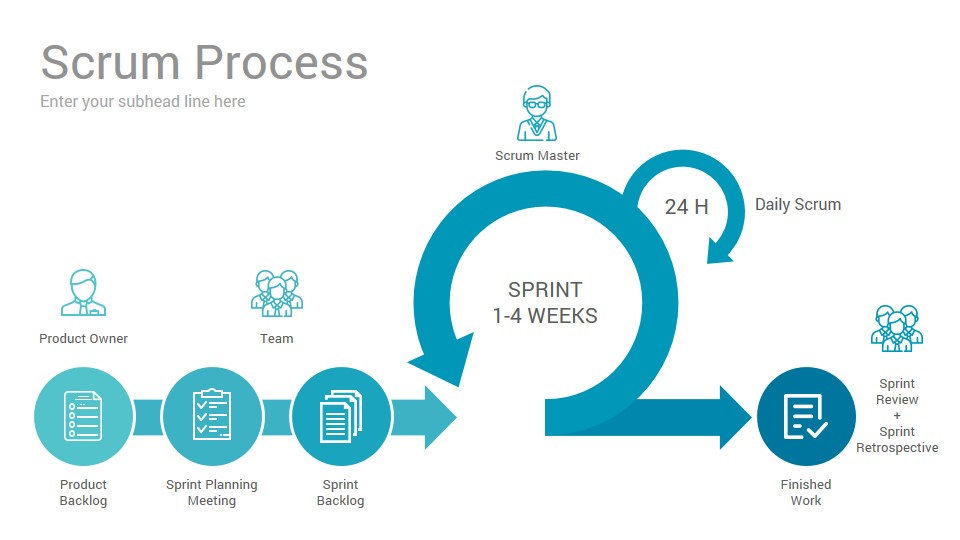
\includegraphics[scale=.4]{propuestaSolicion/turismo/images/metodologiaScrum}
			\caption{Metodología SCRUM}
		}
		\label{fig:metodologiaScrum}
	\end{center}
\end{figure}

En la Figura \ref{fig:metodologiaScrum}: \hyperlink{fig:metodologiaScrum}{Metodología SCRUM}, se muestran las principales actividades que se deben llevar a cabo en la metodología SCRUM. \\

Para el desarrollo del presente proyecto se definirá una etapa de análisis de requerimientos que nos genere la base técnica para el desarrollo del proyecto, sus condiciones y reglas de negocio. Así mismo definiremos 7 sprints para generar prototipos por cada uno de los módulos que conforman el sistema, los cuales son: \\

\begin{itemize}
	\item Sprint 1: Análisis, diseño y desarrollo del módulo \textbf{Registro}
	
	\item Sprint 2: Análisis, diseño y desarrollo del módulo \textbf{Posicionamiento}
	
	\item Sprint 3: Análisis, diseño y desarrollo del módulo \textbf{Localización de rutas}
	
	\item Sprint 4: Análisis, diseño y desarrollo del módulo \textbf{Interacción de la información}
	
	\item Sprint 5: Análisis, diseño y desarrollo del módulo \textbf{Servicios}
	
	\item Sprint 6: Análisis, diseño y desarrollo del módulo \textbf{Información y representación de rutas turísticas}
	
	\item Sprint 7: Análisis, diseño y desarrollo del módulo \textbf{Registro Área Turística}
	
\end{itemize}

Cabe mencionar que al finalizar cada sprint vendrá una etapa de pruebas del sprint desarrollado. 
